\documentclass{beamer}
\usepackage{amsmath, amsthm, amssymb}
\usepackage{enumitem}
\usepackage{tcolorbox}
\usetheme{boadilla}
\makeatother
\setbeamertemplate{footline}
{
  \leavevmode%
  \hbox{%
  \begin{beamercolorbox}[wd=.5\paperwidth,ht=2.5ex,dp=1ex,center]{author in head/foot}%
    \usebeamerfont{author in head/foot}\insertshortauthor
  \end{beamercolorbox}%
  \begin{beamercolorbox}[wd=.5\paperwidth,ht=2.5ex,dp=1ex,center]{title in head/foot}%
    \usebeamerfont{title in head/foot}\insertshorttitle\hspace*{1em}
    \insertframenumber{} / \inserttotalframenumber\hspace*{1ex}
  \end{beamercolorbox}}%

  \vskip0pt%
}
\makeatletter
\setbeamertemplate{navigation symbols}{}
\setitemize{label=\usebeamerfont*{itemize item}%
  \usebeamercolor[fg]{itemize item}
  \usebeamertemplate{itemize item}}

% Setting up a better font
\usefonttheme{professionalfonts}
\usefonttheme{serif}

\title{Query Complexity of Mastermind Variants}
\author{Aaron Berger, Christopher Chute, Matthew Stone}

\begin{document}
    \begin{frame}
    	\maketitle
    \end{frame}

    \begin{frame}
    	\frametitle{Mastermind}
	   	\begin{enumerate}[label=\roman*.]
	    \item Codemaker vs. Codebreaker
	    \item Queries: Guess a vector from $\{1,2,\ldots,6\}^4$.	    		    
	    \item Response
	    	\begin{enumerate}[label=\roman*.]
			\item Black hits
			\item White hits
			\end{enumerate}
   	    \end{enumerate}
	\begin{center}
	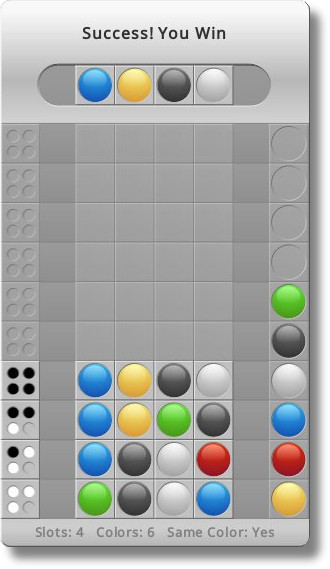
\includegraphics[width=.25\textwidth]{mm.jpg}
	\end{center}
    \end{frame}

    \begin{frame}
    	\frametitle{Knuth Paper -- 1976}
		At most five turns needed to guarantee a victory\vspace{\baselineskip}
		\begin{tcolorbox}[colback=green!5,colframe=green!40!black,title=Minimax]
		For each possible guess
			\begin{enumerate}[label=]
			\item For each possible response to that guess
				\begin{enumerate}[label=]
				\item Check how many possible solutions remain
				\end{enumerate}
			\item Let \textit{score} be min. number solutions eliminated
			\end{enumerate}
		Make guess with maximum score
		\end{tcolorbox}
    \end{frame}
 
    \begin{frame}
    	\frametitle{Optimality of the Minimax Algorithm}
	\begin{tcolorbox}[colback=blue!5,colframe=blue!40!black,title=Lemma (Pigeonhole Principle)]
	For a query with $r$ possible responses, there exists a response that would leave
	at least $1/r$ of possible solutions remaining.
	\end{tcolorbox}
	Analyze the worst-case performance of any algorithm. \\
		\begin{enumerate}[label=\roman*.]
		\item Worst case response to first guess $\Rightarrow$ At least 256 solutions
		remain.
		\item Second guess:  At least $\lceil 256/14 \rceil = 19$ solutions remain.
		\item Third guess: At least $\lceil 19/14 \rceil = 2$ solutions remain
		\item Fourth guess: At least two possible solutions left $\Rightarrow$ cannot
		guarantee to guess the solution on the fourth turn.
		\end{enumerate}
    \end{frame}

    \begin{frame}
    	\frametitle{Extensions}
		\begin{enumerate}[label=\roman*.]
		\item Basic Extension: $n$ spots, $k$ colors
		\item Repeats vs. no repeats
		\item Non-adaptive vs. adaptive strategies
		\end{enumerate}
    \end{frame}
    
    \begin{frame}
    \frametitle{Trivial Lower Bound}
    \begin{tcolorbox}[colback=blue!5,colframe=blue!40!black,title=Theorem]
	\textit{(Game: $n$ spots, $k$ colors, repeats, adaptive allowed).}
	For any strategy that guarantees a win in $s$ turns,
		\begin{equation*}
		s\ge O\left(\frac{n\log k}{\log n^2}\right)
		\end{equation*}
	\end{tcolorbox}
%	\onslide<2->{Recall Lemma:
%	For a query with $r$ possible responses, there exists a response that would leave
%	at least $1/r$ of the possible solutions remaining.
%    \begin{itemize}}
%	\onslide<3->{\item \# of solutions = $k^n$.}
%	\onslide<4->{\item $\binom{n+2}{2} \approx n^2$ possible responses per turn.
%    \end{itemize}}
%	\onslide<5->{In worst case, we need $\le 1$ possible solution remaining.\\
%	$\Longrightarrow$ For any strategy that guarantees a win in $s$ turns,
%		\begin{equation*}
%		\frac{k^n}{\binom{n+2}{2}^s} \leq 1
%		\end{equation*}}
%	\end{frame}
% SEQUENCE OF RESPONSES METHOD
	\begin{proof}
    \begin{enumerate}[label=\arabic*.]
	\onslide<2->{\item Winning Condition: Distinct sequence of responses for each of
	$k^n$ vectors. Let $s$ be number of guesses to guarantee a win.}
	\onslide<3->{\item $\binom{n+2}{2}$ possible responses (cf. stars and bars),
	giving $\binom{n+2}{2}^s$ possible response sequences.}
	\onslide<4->{\item Therefore, $s$ must satisfy
		\begin{equation*}
		\binom{n+2}{2}^s\ge k^n
		\end{equation*}}
	\end{enumerate}
	\end{proof}
	\end{frame}

    \begin{frame}
    \frametitle{(Somewhat) Trivial Upper Bound}
    \begin{enumerate}[label=\arabic*.]
	\item Represent guesses and solutions as matrices ($Q_{ij} = 1$ iff the i-th spot is the j-th color) \\
	\begin{tcolorbox}[colback=blue!5,colframe=blue!40!black,title=Example]
	The guess $(1,1,3)$ would become:
	\[ \left( \begin{array}{ccc}
	1 & 0 & 0 \\
	1 & 0 & 0 \\
	0 & 0 & 1 \end{array} \right)\]
	\end{tcolorbox}
	\onslide<2->{\item $Q_{ij} \in \mathbb R^{nk}$}
	\onslide<3->{\item \# of black hits of $Q$ with hidden matrix $X$ is  $Q\cdot X$.}
	\onslide<4->{\item Guess a basis of span of all such matrices ($\le nk$ guesses)}
	\onslide<5->{\item Dot products with basis $\Rightarrow$ Uniquely determine $ X$} \vspace{10px}
    \end{enumerate}
    \end{frame}

    \begin{frame}
    \frametitle{(Somewhat) Trivial Upper Bound}
	 \begin{enumerate}[label=\arabic*.]
	\item Represent guesses and solutions as matrices ($Q_{ij} = 1$ iff the i-th spot is the j-th color) \\
	\begin{tcolorbox}[colback=blue!5,colframe=blue!40!black,title=Example]
	The guess $(1,1,3)$ would become:
	\[ \left( \begin{array}{ccc}
	1 & 0 & 0 \\
	1 & 0 & 0 \\
	0 & 0 & 1 \end{array} \right)\]
	\end{tcolorbox}
	\begin{tcolorbox}[colback=blue!5,colframe=blue!40!black,title=Theorem]
	There exists a set of at most $nk$ guesses such that any hidden vector is uniquely determined by the responses
	to those guesses.
	\end{tcolorbox} 
	\end{enumerate}
    \end{frame}


%    \begin{frame}
 %   \frametitle{Coin-Weighing Problem}
%    [Grebinski \& Kucherov, 2000], [Bshouty, 2009]
%    \begin{enumerate}[label=\roman*.]
%		\item Original Coin-Weighing algorithm by G\&K, non-constructive (probabilistic method)
%		\item Refined polynomial-time algorithm [Bshouty]
%	\end{enumerate}
%    [Doerr et. al., 2013]
%    	\begin{enumerate}[label=\roman*.]
%		\item Split hidden vector into ``coins'' (subvectors).
%		\item ``Weight" of each ``coin" is \# of black hits.
%		\item Use coin weighing algorithm to eliminate colors.
%		\end{enumerate}
%    \end{frame}

    \begin{frame}
    \frametitle{Entropy Method}
    \textit{Surprise Function:} For an event $x$, we want
	\begin{tcolorbox}[colback=blue!5,colframe=blue!40!black,title=Definition (Surprise Function)]
    	\begin{enumerate}[label=\arabic*.]
		\onslide<2->{\item $S(x) = 0$ when $\mathbb{P}[x]=1$}
		\onslide<3->{\item $S(x) = 1$ when $\mathbb{P}[x]=1/2$}
		\onslide<4->{\item Decreasing function of $\mathbb{P}[x]$}
		\onslide<5->{\item $S(x \land y)=S(x)+S(y|x)$\quad ($=S(x)+S(y)$ if independent)}
	\end{enumerate}
	\end{tcolorbox}

	\onslide<6->\begin{tcolorbox}[colback=blue!5,colframe=blue!40!black,title=Unique Surprise Function]
	$S(x)=-\log_2(\mathbb{P}[x])$.
	\end{tcolorbox}
	\end{frame}
	
	\begin{frame}
	\frametitle{Entropy Method}
	Entropy is the expected surprise of a random variable. \\ \vspace{\baselineskip}
	\onslide<2->\begin{tcolorbox}[colback=blue!5,colframe=blue!40!black,title=Definition (Entropy)]
	Let $X$ be a random variable with domain $D$.
			\begin{equation*}
			H(X) = \sum_{x\in D}\mathbb{P}[X=x]\cdot(-\log_2\left(\mathbb{P}[X=x]\right))
			\end{equation*}
	\end{tcolorbox}
    \end{frame}
 
    \begin{frame}
    \frametitle{Entropy Method}
	\begin{tcolorbox}[colback=blue!5,colframe=blue!40!black,title=Lemma]
	A single turn in a non-adaptive strategy has $<$ $4$ bits of entropy.
	\end{tcolorbox}
	\onslide<2->
	\begin{tcolorbox}[colback=blue!5,colframe=blue!40!black,title=Lemma]
	The number of bits of entropy in any winning strategy is exactly 
	\begin{equation*}
	\log_2 \left(\frac{k!}{(k-n)!}\right).
	\end{equation*}
	\end{tcolorbox}
	\onslide<3->
	\begin{tcolorbox}[colback=blue!5,colframe=blue!40!black,title=Theorem]
	The number of queries submitted by any winning non-adaptive strategy is at least
	\begin{equation*}
	\frac{1}{4}\log_2 \left(\frac{k!}{(k-n)!}\right).
	\end{equation*}
	\end{tcolorbox}
    \end{frame}
   
    \begin{frame}
    \frametitle{Probabilistic Method}
    Choose a random set of queries $Q=\{q_1, q_2, \ldots, q_s\}$. \\ \vspace{5px}
    Calculate $\mathbb{P}[Q\text{ is a winning set of guesses}]$ \vspace{5px}
    \onslide<2->
    \begin{tcolorbox}[colback=blue!5,colframe=blue!40!black,title=Theorem]
	When the random set of guesses is of magnitude $s = 4k \log k$
    	\begin{align*}
		\mathbb{P}[Q\text{ is a win} & \text{ning set of guesses }] > 0 \\
		\onslide<3->{& \Downarrow \\
		\exists \text{ a winning } & \text{set of $4k \log k$ guesses}}
	\end{align*}
    \end{tcolorbox}
    \end{frame}

\begin{frame}
\frametitle{Thanks!}
	\begin{enumerate}[label=\arabic*.]
	\item Special thanks to Danny Montealegre, Nathan Kaplan.
	\item Thanks to SUMRY for this research opportunity.
	\item Thanks to MathFest for the opportunity to present.
	\end{enumerate}
\end{frame}

%    \begin{frame}
%    \frametitle{Future Topics to Explore}
%    \begin{enumerate}[label=\arabic*.]
%	\item $k>n$: no tight bounds
%	\item Permutation game algorithms
%	
%    \end{enumerate}
%    \end{frame}

\end{document}





























